\chapter{质点运动学}
质点运动学是研究质点运动规律的物理学分支,涉及质点的位移、速度、加速度等基本概念及其运动方程。

\marginnote[-17em]{
\indent
\key{质点:}忽略物体的形状和大小,只考虑物体的质量和位置的理想化物理模型。

\key{参考系:}观测者参考系或观察和描述物体运动的坐标系。

{\scriptsize \rmit{\quad 高中物理所谓参考系,通常是指观测者参考系中的惯性参考系。}}

\key{矢量:}既有大小又有方向的物理量

\key{标量:}只有大小没有方向的物理量。
}


\section{位矢,位移,速度,加速度}

\begin{marginfigure}[4.5cm]
    \includegraphics{/Position Vector/G-1/G1.pdf}
    \caption[Position vector]{
        位矢,位移,速度,加速度\\
        }
    \label{fig:Position Vector_G1}
\end{marginfigure}

\key{位矢:}位置矢量的简称,指从参考系原点指向质点位置的矢量。
记作$r$,质点的运动就用位矢随时间的变化来描述,即
$$
r = r(t)
$$

\key{位移:}指物体在参考系中从初位置到末位置的有向线段。
记作$\Delta r$,显然有
$$
\Delta r = r(t+\Delta t) - r(t)
$$

{\small
高中人教版物理,位移常表示为$\Delta x$。
}
\vspace{1em}

\key{速度:}指物体在单位时间内的位移量,即位矢的时间变化率。
记作$v$,显然有
$$
v = \lim_{\Delta t \to 0} \frac{r(t+\Delta t) - r(t)}{\Delta t}
= \lim_{\Delta t \to 0} \frac{\Delta r}{\Delta t}
= \frac{\textup{d} r}{\textup{d}t}
$$

\key{加速度:}指物体在单位时间内的速度变化量,即速度的时间变化率,显然有
$$
a = \lim_{\Delta t \to 0} \frac{v(t+\Delta t) - v(t)}{\Delta t}
= \lim_{\Delta t \to 0} \frac{\Delta v}{\Delta t}
= \frac{\textup{d} v}{\textup{d}t}
$$



\section{直角坐标系}
这里仅介绍直角坐标系及其变换,其他坐标系(如极坐标系、柱坐标系、球坐标系等)将在后续章节中介绍。
\begin{figure}
    \includegraphics[width=0.8\textwidth, keepaspectratio]{/Coordinate System/G-1/G1.pdf}
    \caption[Cartesian coordinate system]{
        直角坐标系\\
        \vspace{2cm}
        \normalsize
        基本矢量:${e}_x$,${e}_y$,${e}_z$
        }
    \label{fig:Coordinate System_G1}
\end{figure}


